\documentclass[conference,a4paper]{IEEEtran}

% Escritura mejorada de fórmulas matemáticas
\usepackage{amsmath}

% Inserción de gráficos
\usepackage{graphicx}

% Escritura de pseudocódigo
\usepackage[kw]{pseudo}

% Escritura mejorada de tablas
\usepackage{booktabs}

% Escritura mejorada de citas bibliográficas
\usepackage{cite}


% Macros traducidas
\def\contentsname{Índice general}
\def\listfigurename{Índice de figuras}
\def\listtablename{Índice de tablas}
\def\refname{Referencias}
\def\indexname{Índice alfabético}
\def\figurename{Fig.}
\def\tablename{TABLA}
\def\partname{Parte}
\def\appendixname{Apéndice}
\def\abstractname{Resumen}
% IEEE specific names
\def\IEEEkeywordsname{Palabras clave}
\def\IEEEproofname{Demostración}


\begin{document}

\title{Algoritmos genéticos para problemas de regresión no lineal.}

\author{
  \IEEEauthorblockN{Javier Santos Martín}
  \IEEEauthorblockA{
    \textit{Dpto. Ciencias de la Computación e Inteligencia Artificial}\\
    \textit{Universidad de Sevilla}\\
    Sevilla, España\\
    javier.jsm21@gmail.com | javsanmar5@alum.us.es}
  
  \and
  
  \IEEEauthorblockN{Javier Ruíz Garrido}
  \IEEEauthorblockA{
    \textit{Dpto. Ciencias de la Computación e Inteligencia Artificial}\\
    \textit{Universidad de Sevilla}\\
    Sevilla, España\\
    jrg@gmail.com | javruigar2@alum.us.es}
}

\maketitle


% Resumen
\begin{abstract}
  Escribir aquí dos párrafos indicando el objetivo principal del trabajo, y un
  resumen de las conclusiones obtenidas. Cabe mencionar que este documento se
  ha confeccionado siguiendo el formato de conferencias de IEEE (ver la guía
  para autores para más información, existen plantillas para Word y \LaTeX).
  Este documento se debe emplear como guía, se pueden añadir nuevas secciones
  según sea necesario. Es importante dotarlo de un número razonable de
  referencias bibliográficas.
\end{abstract}


% Palabras claves
\begin{IEEEkeywords}
  Inteligencia Artificial, otras palabras clave…
\end{IEEEkeywords}


\section{Introducción}

En esta sección se dedican varios párrafos para dar el contexto en el que se
desarrolla el trabajo presentado. Normalmente se va desde lo más general a lo
más preciso, para englobar el trabajo dentro de un ámbito concreto. Hay que
recordar que se debe referenciar la información que se consiga de fuentes
bibliográficas (artículos, libros, capítulos de libros, páginas web, apuntes,
etc.). Para ello se añade el ítem correspondiente en el apartado de
referencias, dotándolo de un número, y se añade la referencia al final de la
frase o párrafo correspondiente~\cite{b1}. Si se realiza en Microsoft Word o
LibreOffice, se puede hacer uso de \emph{referencias cruzadas} para actualizar
la numeración de las referencias de forma automática en todo el documento.

Después vienen un par de párrafos para dar un poco más de detalle sobre el
trabajo realizado. Hay que indicar la problemática o el objetivo que se marca,
y cómo se ha enfocado la solución propuesta en este trabajo. Finalmente, el
último párrafo se dedica a comentar la estructura del documento por secciones,
como el que sigue.

\section{Preliminares}

En este trabajo, se busca aplicar la idea de los algoritmos genéticos para resolver problemas de regresión. Para ello, los cromosomas modelarán los parámetros de la función que intentamos predecir, y su valoración se realizará utilizando datos de prueba. Esto se llevará a cabo prediciendo los datos y evaluando la precisión de las predicciones comparándolas con los resultados esperados.

Todo esto se desarrollará dentro de un algoritmo genético estándar, que incluirá componentes como el elitismo, el cruce entre cromosomas y la mutación aleatoria. Finalmente, se explicarán algunas medidas para mejorar la eficiencia en este contexto específico.

\subsection{Cromosoma}

\subsubsection{Propiedades}
\begin{itemize}
    \item \textbf{Lista de coeficientes:} Esta lista contiene \( n + 1 \) elementos de tipo \texttt{float}, donde \( n \) es el número de variables independientes. El elemento \( j \) de la lista representa el coeficiente de la variable \( x_j \), mientras que el último elemento representa el término independiente.
    \item \textbf{Lista de exponentes:} Esta lista contiene \( n \) elementos de tipo \texttt{float}, donde \( n \) es el número de variables independientes. El elemento \( j \) de la lista representa el exponente de la variable \( x_j \).
\end{itemize}

Aunque, a priori, todos los elementos de ambas listas no tienen restricciones en cuanto a los valores que pueden adoptar, existen dos situaciones que podrían limitar estos valores:


1. \textbf{Variable \( x_i \) negativa:} En este caso, el exponente de la función no puede asumir valores fraccionarios cuyo denominador sea par, es decir, de la forma \( k/m \) donde \( m \) es par, en el ámbito de los números reales. Este hecho plantea un problema en Python, ya que cualquier número negativo elevado a una potencia fraccionaria, ya sea con un denominador par o impar, resulta en un número complejo. Esto no es deseable, dado que estamos trabajando en el conjunto de los números reales \( \mathbb{R} \). Podemos ver este fallo de Python ejemplificado a continuación, donde se eleva un número negativo \( -1 \) a un número fraccionario con denominador impar \( 0.2 = \frac{1}{5} \), lo que resulta en la raíz quinta de \(-1\), que es igual a \(-1\):

Esperado:
\[
\sqrt[5]{-1} = -1
\]

Obtenido:
\begin{verbatim}
>>> base, exponent = -1, 0.2
>>> base ** exponent
(0.8090169943749475+0.5877852522924731j)
\end{verbatim}

Para resolver este problema, hemos decidido redondear los exponentes a su parte entera en los casos donde surge esta dificultad. Esta decisión se tomó después de descartar otras opciones, como intentar modificar la fracción para garantizar que el denominador sea impar (lo cual hemos observado que no es efectivo por el error de Python) o alterar la base (representada por la variable \(x_j\)), lo cual consideramos completamente incorrecto. Modificar la base implicaría permitir exponentes que generan este problema y exigiría a quienes utilicen esta solución que ajusten sus variables para trabajar con números positivos. Además, sabemos que si alteramos la base, es decir, los datos de entrada, el valor esperado \(y_i\) ya no sería válido, dado que el dato de entrada no sería el original.




2. \textbf{Variable \( x_i \) igual a cero:} Aquí, el problema surge con los exponentes negativos, pues esta operación está indeterminada. Por tanto, para resolver este problema, utilizamos el valor absoluto del exponente, ya que al saber que la función a interpolar está definida en \( x_i = 0 \), podemos afirmar que \( e_j > 0 \).


\subsubsection{Fitness}
En esta sección, se realizará la evaluación de los cromosomas. Una idea fundamental en los algoritmos genéticos es la capacidad de valorar con la mayor precisión posible cada cromosoma, con el objetivo de determinar si un cromosoma es mejor o peor que otro. En el contexto de un problema de regresión, esta evaluación se basa en la comparación entre los valores predichos por el cromosoma y los valores reales.

Para evaluar la precisión de las predicciones, utilizamos el error cuadrático medio (RMSE, por sus siglas en inglés), una métrica ampliamente aceptada en problemas de regresión. El RMSE se calcula mediante la siguiente fórmula:

\[
\text{RMSE} = \sqrt{\frac{\sum_{i=1}^{N} (y_i - \hat{y}_i)^2}{N}}
\]

donde \( y_i \) representa los valores reales y \( \hat{y}_i \) las predicciones realizadas por el cromosoma, y \( N \) es el número total de datos.

Una vez calculado el RMSE para un cromosoma específico, existen dos enfoques posibles para su utilización en la función de fitness: devolver el inverso del RMSE para maximizar el valor de la función de fitness, o devolver el RMSE directamente y minimizar su valor. En nuestro caso, hemos optado por la segunda opción, es decir, minimizar el RMSE.

A continuación, describiremos el proceso de predicción utilizando los datos del cromosoma en cuestión, que es crucial para la evaluación de su fitness.

\subsubsection{Predicción}
En esta sección, explicaremos cómo obtener una predicción \(\hat{y}_i\) para un cromosoma específico utilizando datos de prueba concretos. Este proceso se repetirá para cada uno de los datos de prueba que deseamos evaluar. Dado que estamos abordando un problema de regresión no lineal, debemos elevar cada una de las variables de los datos de prueba \(x_j\) a un exponente \(e_j\) y multiplicarlas por un coeficiente \(c_j\), donde \(j\) representa los índices de todas las variables en la ecuación de regresión. 

Posteriormente, sumamos estos términos junto con un último coeficiente, que actúa como término independiente, para obtener la predicción final. Utilizando los valores de un cromosoma determinado, la predicción \(\hat{y}_i\) se calcula de la siguiente manera:

\[
\hat{y}_i = \sum_{j=0}^{n} c_j x_j^{e_j} + c_{n+1}
\]


\subsubsection{Cruce de Cromosomas}
El proceso de cruce de cromosomas tiene como objetivo combinar dos cromosomas parentales, eligiendo un punto de cruce de manera aleatoria. Una vez determinado el punto de cruce, se crean dos cromosomas hijos seleccionando una parte del cromosoma de cada padre. 

Para decidir cuándo realizar el cruce, se utiliza una tasa de cruce, la cual es un valor entre 0 y 1. Se elige un número aleatorio, también entre 0 y 1, y la probabilidad de que este número sea menor que la tasa de cruce es precisamente la tasa de cruce. Por lo tanto, si el número aleatorio es mayor que la tasa de cruce, los cromosomas se devuelven sin cambios. 

En caso de que se deba realizar el cruce, se genera aleatoriamente un punto de corte en los cromosomas parentales. En este punto, ambos cromosomas se dividen y se combinan emparejando una mitad de uno con la mitad complementaria del otro, y viceversa. Podemos ver este proceso ejemplificado en \figurename~\ref{fig:chromosome-crossover}


\begin{figure}[h]
    \centering
    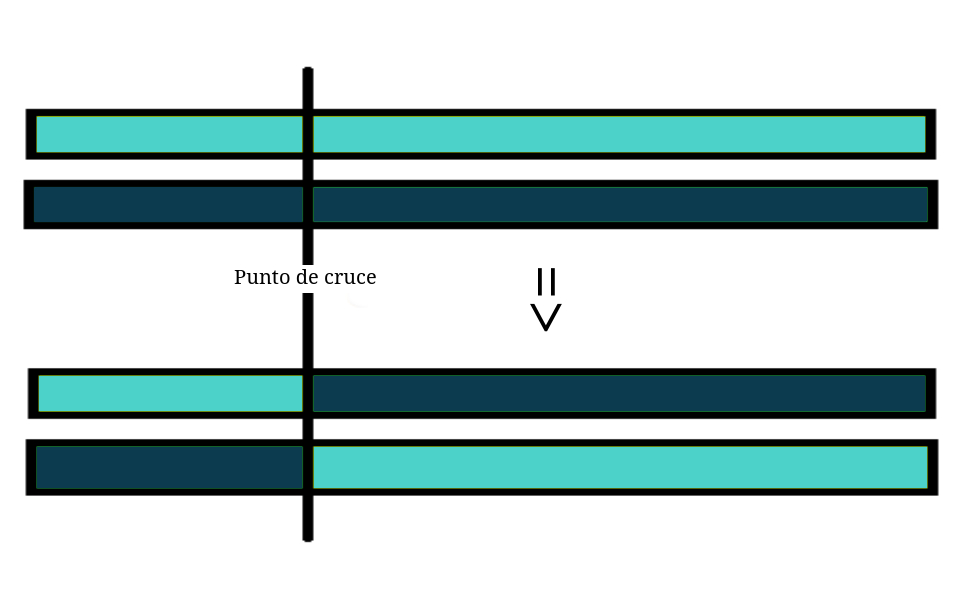
\includegraphics[width=\columnwidth]{image-chromosome-crossover.jpg}
    \caption{Proceso de cruce ilustrado.}
    \label{fig:chromosome-crossover}
\end{figure}


En nuestro caso, dado que manejamos dos listas, una de coeficientes y otra de exponentes, se generan dos puntos de corte y se realiza el cruce de la manera descrita anteriormente en ambas listas. Creando dos nuevos objetos Cromosoma, y devolviendo estos dos.



\subsubsection{Mutación de Cromosomas}
La mutación de cromosomas se realiza de manera aleatoria, similar al proceso de cruce de cromosomas. Este proceso utiliza una tasa de mutación, la cual es un valor entre 0 y 1. Para cada parámetro del cromosoma, se genera un número aleatorio, también entre 0 y 1. Si este número es menor que la tasa de mutación, se decide mutar el parámetro correspondiente.

Cuando un parámetro es seleccionado para mutación, se modifica sumándole un valor aleatorio dentro de un rango predeterminado. Este rango incluye números negativos, por lo que el parámetro puede incrementarse o disminuirse con igual probabilidad. 

Este proceso se aplica a cada parámetro del cromosoma. Una vez realizado a todos estos, finaliza el proceso de mutación.


\subsection{Algoritmo Genético}
En esta sección, describimos el proceso completo del algoritmo genético, utilizando los componentes definidos anteriormente. El algoritmo comienza con la generación de una población inicial de un tamaño determinado. Cada cromosoma de la población es evaluado utilizando la función de fitness descrita previamente.

Una vez que todos los cromosomas han sido evaluados, se ordenan de menor a mayor según su valor de fitness, y se seleccionan los mejores para formar la población de la siguiente generación. Con los cromosomas restantes, se procede de la siguiente manera:

\subsubsection{Selección Mediante Torneo}
Para seleccionar los padres de la siguiente generación, se utiliza un método de selección mediante torneo. Este proceso consiste en seleccionar aleatoriamente \(k\) cromosomas y escoger los dos con mejor fitness, es decir, los dos con el menor RMSE respecto a los datos reales.

Una vez seleccionados los dos padres, se generan dos hijos para la siguiente generación utilizando el proceso de cruce explicado anteriormente. Posteriormente, estos hijos pasan por un proceso de mutación aleatoria. 

Este ciclo se repite tantas veces como el número de iteraciones especificado. Al finalizar la última iteración, se devuelve el cromosoma con el menor RMSE como la solución final al problema.


\subsection{Medidas para Mejorar la Eficiencia}
Además de buscar el menor RMSE posible, también teníamos la intención de optimizar los tiempos de ejecución de nuestro algoritmo, de manera que pudiera llegar a soluciones esperadas en el menor tiempo posible. Para alcanzar este objetivo, hemos implementado varias medidas destinadas a mejorar la eficiencia del algoritmo. Estas medidas son:

\subsubsection{Porcentaje de Datos}
En principio, cuantos más datos tengamos en nuestro conjunto de prueba, mejor, ya que esto proporcionará una mayor variedad en nuestro proceso de valoración y, en general, conducirá a una regresión más precisa. Sin embargo, al aumentar el número de casos de prueba, también aumenta el tiempo necesario para valorar cada cromosoma. 

Con el fin de aprovechar las ventajas de tener un gran número de datos de prueba, pero reduciendo el costo computacional, proponemos la siguiente solución: introducir un nuevo parámetro, con un valor entre 0 y 1, que indique el porcentaje de datos a utilizar. Estos datos se seleccionarán de forma aleatoria para cada valoración de un cromosoma. 

De esta manera, un cromosoma que progresa a través de distintas generaciones debido a su buen desempeño en los datos que le han tocado, será evaluado con diferentes subconjuntos de datos en cada iteración. Esto no solo asegura una evaluación más robusta, sino que también reduce significativamente el costo computacional de valorar un cromosoma.

\subsubsection{Almacenamiento de la Valoración de un Cromosoma}
Durante la ejecución del algoritmo genético, debemos ordenar todos los cromosomas de la población actual en función de su valoración. Estas valoraciones también se utilizan posteriormente en la selección por torneo.

Inicialmente, la población se representaba como una lista de cromosomas, y el cálculo de la valoración se realizaba cada vez que era necesario obtener la valoración de un cromosoma. Este enfoque era extremadamente ineficiente.

Para mejorar la eficiencia, propusimos cambiar esta lista de cromosomas por una lista en la que se almacenen pares \([\text{cromosoma}, \text{cromosoma.fitness()}]\). Consideramos varias opciones para implementar esta estructura, y finalmente optamos por utilizar una lista de listas. Aunque esta elección podría ser ligeramente menos eficiente que usar un diccionario o una lista de tuplas, vimos que la manipulación de listas era lo más comodo para nosotros. Las listas son variables mutables, lo que nos permite crear la población de la siguiente generación y realizar operaciones de mutación y cruce con facilidad. Al comienzo de cada nueva generación, podemos establecer las valoraciones utilizando nuevos datos de prueba, tal como se explicó anteriormente.


\section{Metodología}

Esta sección se dedica a la descripción del método implementado en el trabajo.
Esta parte es la correspondiente a lo realmente desarrollado en el trabajo, y
se puede emplear pseudocódigo (nunca código), esquemas, tablas, etc.

A continuación, un ejemplo de uso de listas numeradas:
\begin{enumerate}
\item\label{item:dos-alumnos} \textit{Trabajos con dos alumnos:} poner nombre y
  apellidos completos de cada uno, y correos electrónicos de contacto (a ser
  posible de la Universidad de Sevilla). El orden de los alumnos se fijará por
  orden alfabético según los apellidos.
\item \textit{Trabajo con un autor:} cambiar la cabecera de la siguiente manera
  \begin{enumerate}
  \item \textit{Una sola columna:} solo se debe especificar un alumno.
  \item \textit{Información a añadir:} la misma que la especificada en el
    punto~\ref{item:dos-alumnos}.
  \end{enumerate}
\end{enumerate}

Las figuras se deben mencionar en el texto, como la
\figurename~\ref{fig:ejemplo}. También se pueden añadir ecuaciones, como la
ecuación~\eqref{eq:ejemplo}.

\begin{equation}
  \label{eq:ejemplo}
  a + b = \gamma
\end{equation}

Un ejemplo de pseudocódigo se puede observar en la
\figurename~\ref{pcd:fitness}.

\begin{figure}[h]
  \centering
  \begin{pseudo}*
    \hd{\fn{fitness}}(self, train\_data, data\_percentage) \\*
    \multicolumn{2}{l}{\textbf{Entrada}: El cromosoma actual, una lista de tuplas de} \\*
    \multicolumn{2}{l}{floats que representan los datos de entrenamiento y un} \\*
    \multicolumn{2}{l}{ float que representa el porcentaje de datos con los que} \\*
    \multicolumn{2}{l}{ será entrenado el cromosoma} \\*
    \multicolumn{2}{l}{\textbf{Salida}: Un float que representa el error cuadrático medio} \\*
    \multicolumn{2}{l}{ (RMSE)} \\
    \fn{y\_pred \(\leftarrow\) lista vacía} \\
    \fn{y\_true \(\leftarrow\) lista vacía} \\
    \fn{selected\_data \(\leftarrow\)} seleccionar aleatoriamente \\+
    \fn{(train\_data * data\_percentage) elementos de} \\+
    \fn{train\_data} \\--
    \textbf{para cada} \fn{datum} \textbf{en} \fn{selected\_data} \textbf{hacer} \\+
    agregar \fn{llamada a la funcion predict con datum} \\+ \fn{como parametro} a \fn{y\_pred} \\
    agregar \fn{último elemento de datum} a \fn{y\_true} \\-
    \fn {rmse} \(\leftarrow\) \fn{root\_mean\_squared\_error}(y\_true, y\_pred) \\
    \textbf{devolver} \fn{rmse}
  \end{pseudo}
  \caption{Función de evaluación del cromosoma (\texttt{fitness}) en pseudocódigo}
  \label{pcd:fitness}
\end{figure}


\begin{figure}[h]
  \centering
  \begin{pseudo}*
    \hd{\fn{predict}}(\textit{self, datum}) \\*
    \multicolumn{2}{l}{\textbf{Entrada}: El cromosoma actual, una tupla de floats que} \\*
    \multicolumn{2}{l}{representa una línea de los datos de entrenamiento} \\*
    \multicolumn{2}{l}{\textbf{Salida}: Un float que representa el valor predicho} \\
    \fn{prediction \(\leftarrow\) 0} \\
    \textbf{para cada} \fn{i} \textbf{en rango} \fn{len(datum) - 1} \textbf{hacer} \\+
    \textbf{si} \fn{\textit{el dato recibido i}} es menor que \fn0
    \textbf{entonces} \\+
    \fn{\textit{el exponente i}} \(\leftarrow\) 
    (redondear a entero \fn{\textit{el}}\\+
    \fn{\textit{ exponente i}} \\--
    \textbf{si no, si} \fn{\textit{el dato recibido i}} es igual que \fn0 \textbf{entonces} \\+
    \textit{\fn{el exponente i}} \(\leftarrow\) \fn{hacer el valor absoluto} \\-
    \fn{exponent \(\leftarrow\) \textit{el exponente i}} \\
    \fn{prediction} \(\mathrel{+}= \textit{\fn{el coeficiente i}} \times \fn{\textit{(el dato recibido i }} \\+
    \text{ elevado a} \fn{exponent)}\) \\--
    \fn{prediction} \(\mathrel{+}= \textit{ \fn{el último coeficiente}}\) \\
    \textbf{devolver} \fn{prediction}
  \end{pseudo}
  \caption{Función de predicción (\texttt{predict}) en pseudocódigo}
  \label{pcd:predict}
\end{figure}



\begin{figure}[h]
  \centering
  \begin{pseudo}*
    \hd{\fn{crossover}}(\textit{self}, \textit{chromosomeToCrossWith}, \textit{cross\_rate}) \\*
    \multicolumn{2}{l}{\textbf{Entrada}: El cromosoma actual, el cromosoma para cruzar y la} \\*
    \multicolumn{2}{l}{ tasa de cruce} \\*
    \multicolumn{2}{l}{\textbf{Salida}: Una lista de los dos cromosomas resultantes del cruce} \\
    \textbf{si \fn{el número random generado} es mayor que } \textit{\fn{cross\_rate}} \\+
    \textbf{entonces} \\+
    \textbf{devolver \fn{una lista con el cromosoma actual y el}} \\+
    \fn{cromosoma con el que iba a ser cruzado} \\---
    \fn{punto} \(\leftarrow\) \fn{número random entre el uno y la longitud de } \\+
    \fn{la lista de exponentes menos uno} \\---
    \fn{child1\_coefficients} \(\leftarrow\)
    \textit{\fn{los coeficientes del cromosoma actual}} \\+ 
    \textit{\fn{hasta "punto" + los coeficientes del cromosoma a cruzar}} \\+
     \textit{\fn{desde "punto"}} \\--
    \fn{child2\_coefficients} \(\leftarrow\) \textit{\fn{los coeficientes del cromosoma a cruzar}} \\+ 
    \textit{\fn{hasta "punto" + los coeficientes del cromosoma actual}} \\+
     \textit{\fn{desde "punto"}} \\--
    \fn{child1\_exponents} \(\leftarrow\)
    \textit{\fn{los exponentes del cromosoma actual}} \\+ 
    \textit{\fn{hasta "punto" + los exponentes del cromosoma a cruzar}} \\+
     \textit{\fn{desde "punto"}} \\--
    \fn{child2\_exponents} \(\leftarrow\)
    \textit{\fn{los exponentes del cromosoma a cruzar}} \\+ 
    \textit{\fn{hasta "punto" + los exponentes del cromosoma actual}} \\+
     \textit{\fn{desde "punto"}} \\--
    \textbf{devolver} \fn{lista con el cromosoma child1\_coefficients} \\+
    \fn{y child1\_exponents, y el cromosoma child2\_coefficients} \\+
    \fn{ y child2\_exponents}
  \end{pseudo}
  \caption{Función de cruza (\texttt{crossover}) en pseudocódigo}
  \label{pcd:crossover}
\end{figure}


\begin{figure}[h]
  \centering
  \begin{pseudo}*
    \hd{\fn{mutate}}(\textit{self}, \textit{mutation\_rate}, \textit{mutation\_range}) \\*
    \multicolumn{2}{l}{\textbf{Entrada}: El cromosoma actual, tasa de mutación y rango de} \\*
     \multicolumn{2}{l}{mutación} \\*
    \multicolumn{2}{l}{\textbf{Salida}: Ninguna} \\
    \textit{\fn{random\_number}} \(\leftarrow\) \fn{Número aleatorio entre 0 y 1} \\--
    \textbf{si} \textit{\fn{random\_number} es menor que}  \textit{\fn{mutation\_rate}} \textbf{entonces} \\+
        \textbf{para cada} \textit{\fn{i}} \textbf{en rango} \fn{longitud de la lista de exponentes} \\+
        \fn{ del cromosoma actual }\textbf{hacer} \\+
            \textit{\fn{coeficiente i del cromosoma actual}} \(\mathrel{+}= \fn{un valor}\\+
            \fn{aleatorio entre -mutation\_range y} \\+ \fn{mutation\_range}\) \\--
            \textit{\fn{exponente i del cromosoma actual}} \(\mathrel{+}= \fn{un valor}\\+
            \fn{aleatorio entre -mutation\_range y} \\+ \fn{mutation\_range}\) \\----
        \textit{\fn{último coeficiente del cromosoma actual}} \(\mathrel{+}= \fn{un valor}\\+
            \fn{aleatorio entre -mutation\_range y mutation\_range}\\--
  \end{pseudo}
  \caption{Función de mutación (\texttt{mutate}) en pseudocódigo}
  \label{pcd:mutate}
\end{figure}



\begin{figure}[h]
  \centering
  \begin{pseudo}*
    \hd{\fn{run}}(\textit{self}) \\*
    \multicolumn{2}{l}{\textbf{Entrada}: Instancia de la clase AG} \\*
    \multicolumn{2}{l}{\textbf{Salida}: El cromosoma con la mejor aptitud encontrada y ese} \\*
    \multicolumn{2}{l}{cromosoma sometido a la funcion test} \\
    \textit{\fn{elitism\_count}} \(\leftarrow\) 
    \fn{ratio de elitismo por el tamaño de} \\+
    \textit{\fn{población}}\\--
    \textbf{para} \textit{\fn{generation}} \textbf{en rango} \textit{\fn{máximas iteraciones}} \textbf{hacer} \\+
    \textbf{para} \textit{\fn{pair}} \textbf{en} \textit{\fn{la población actual}} \textbf{hacer} \\+
        \textit{\fn{self.population}} \(\leftarrow\) \(\text{\fn{lista de listas del primer}} \\+
        \fn{elemento de pair y de su función fitness} \\--
        \textit{\fn{self.population}} \(\leftarrow\) 
        \fn{se ordena por el segundo}\\+
        \fn{elemento de cada tupla de la lista de}\\+
        \fn{población} \\--
        \textbf{para} \textit{\fn{pair}} \textbf{en} \textit{\fn{la población actual hasta el}} \\+
        \fn{elitism\_count elemento} \textbf{hacer} \\+
        \textit{\fn{next\_generation}} \(\leftarrow\) \(\text{\fn{añadir el primer}} \\+
        \fn{elemento de pair} \\---
        \textbf{mientras} \fn{longitud de}
        \textit{\fn{next\_generation} menor que} \\+
        \textit{\fn{tamaño de población}} \textbf{hacer} \\+
            \fn{\textit{parent1}, \textit{parent2}} \(\leftarrow\) \fn{cromosoma ganador del} \\+
            \fn{\textit{torneo}, \textit{cromosoma ganador del torneo}} \\-
            \textit{\fn{offspring}} \(\leftarrow\) \textit{\fn{crossover entre parent 1 y 2}}\\
            \textbf{para cada} \textit{\fn{child}} \textbf{en} \textit{\fn{offspring}} \textbf{hacer} \\+
                \textbf{si} \fn{longitud de next\_generation} menor\\+
                que \fn{tamaño población} \\+
                    \fn{\textit{child} \(\leftarrow\) \textit{mutate cromosoma}} \\
                    \fn{\textit{next\_generation}} \(\leftarrow\) \textit{añadir}\\+ \fn{child} \\------
        \fn{\textit{best\_fitness} \(\leftarrow\) \textit{segundo elemento de la primera tupla}}\\+
        \fn{de la lista de población} \\-
        \fn{\textit{self.population} \(\leftarrow\) \textit{next\_generation}} \\-
    \textit{\fn{winner\_chromosome}} \(\leftarrow\) 
    \fn{cromosoma con mejor fitness}\\
    \textbf{devolver} 
    \fn{\textit{winner\_chromosome}, \textit{test de winner\_chromosome}} \\
  \end{pseudo}
  \caption{Función de ejecución (\texttt{run}) en pseudocódigo}
  \label{pcd:run}
\end{figure}


\begin{figure}[h]
  \centering
  \begin{pseudo}*
    \hd{\fn{tournament\_selection}}(\textit{self}, \textit{k}) \\*
    \multicolumn{2}{l}{\textbf{Entrada}: Instancia de la clase AG y número de cromosomas} \\*
    \multicolumn{2}{l}{seleccionados para el torneo (\textit{k})} \\*
    \multicolumn{2}{l}{\textbf{Salida}: Cromosoma con la mejor aptitud} \\
    \textit{\fn{tournament}} \(\leftarrow\) \fn{k elementos aleatorios de población actual}\\--
    \textit{\fn{sorted\_tournament}} \(\leftarrow\) 
        \fn{se ordena por el segundo}\\+
        \fn{elemento de cada tupla de la lista de población}\\--
    \textbf{devolver} \textit{\fn{primer elemento de sorted\_torunament}} \\
  \end{pseudo}
  \caption{Selección de torneo en pseudocódigo}
  \label{pcd:tournament_selection}
\end{figure}




\begin{figure}[h]
  \centering
  \begin{pseudo}*
    \hd{\fn{test}}(\textit{self}, \textit{chromosome}) \\*
    \multicolumn{2}{l}{\textbf{Entrada}: Instancia de la clase AG y cromosoma a probar} \\*
    \multicolumn{2}{l}{\textbf{Salida}: Lista de valores predichos} \\
    \textit{\fn{y\_pred\(\leftarrow\) lista vacía}} \\--
    \textbf{para cada} \textit{\fn{datum}} \textbf{en} \textit{\fn{test\_data}} \textbf{hacer} \\+
        \textit{\fn{predicted \(\leftarrow\) \textit{predict datum}}} \\
        \textit{\fn{y\_pred \(\leftarrow\) \textit{añadir predicted}}} \\--
    \textbf{devolver} \textit{\fn{y\_pred}} \\
  \end{pseudo}
  \caption{Función de prueba (\texttt{test}) en pseudocódigo}
  \label{pcd:test}
\end{figure}










\section{Resultados}

En esta sección se detallarán tanto los experimentos realizados como los
resultados conseguidos:
\begin{itemize}
\item Los experimentos realizados, indicando razonadamente la configuración
  empleada, qué se quiere determinar, y como se ha medido.
\item Los resultados obtenidos en cada experimento, explicando en cada caso lo
  que se ha conseguido.
\item Análisis de los resultados, haciendo comparativas y obteniendo
  conclusiones.
\end{itemize}

Se pueden hacer uso de tablas, como el ejemplo de la tabla~\ref{tab:ejemplo}.

\begin{table}
  \caption{Ejemplo de tabla}
  \label{tab:ejemplo}
  \centering
  \begin{tabular}{ccc}
    \toprule
    A & B & C \\
    \midrule
    1 & 2 & 3 \\
    4 & 5 & 6 \\
    \bottomrule
  \end{tabular}
\end{table}


\section{Conclusiones}

Finalmente, se dedica la última sección para indicar las conclusiones obtenidas
del trabajo. Se puede dedicar un párrafo para realizar un resumen sucinto del
trabajo, con los experimentos y resultados. Seguidamente, uno o dos párrafos
con conclusiones. Se suele dedicar un párrafo final con ideas de mejora y
trabajo futuro.


\begin{thebibliography}{00}
\bibitem{b1} G. Eason, B. Noble, and I. N. Sneddon, ``On certain integrals of Lipschitz-Hankel type involving products of Bessel functions,'' Phil. Trans. Roy. Soc. London, vol. A247, pp. 529--551, April 1955.
\bibitem{b2} J. Clerk Maxwell, A Treatise on Electricity and Magnetism, 3rd ed., vol. 2. Oxford: Clarendon, 1892, pp.68--73.
\bibitem{b3} I. S. Jacobs and C. P. Bean, ``Fine particles, thin films and exchange anisotropy,'' in Magnetism, vol. III, G. T. Rado and H. Suhl, Eds. New York: Academic, 1963, pp. 271--350.
\bibitem{b4} K. Elissa, ``Title of paper if known,'' unpublished.
\bibitem{b5} R. Nicole, ``Title of paper with only first word capitalized,'' J. Name Stand. Abbrev., in press.
\bibitem{b6} Y. Yorozu, M. Hirano, K. Oka, and Y. Tagawa, ``Electron spectroscopy studies on magneto-optical media and plastic substrate interface,'' IEEE Transl. J. Magn. Japan, vol. 2, pp. 740--741, August 1987 [Digests 9th Annual Conf. Magnetics Japan, p. 301, 1982].
\bibitem{b7} M. Young, The Technical Writer's Handbook. Mill Valley, CA: University Science, 1989.
\end{thebibliography}




\end{document}
